% BANKS-SOURCE: pdf=166 print=156 kind=section id=9.6
\subsection{Renormalization of $\phi^4$ field theory}

% BANKS-SOURCE: pdf=166 print=156 kind=prose
We're now ready to do an explicit perturbative example of renormalization. The
CFT of a single free massless scalar has four relevant/marginal perturbations:
$:\phi^n:$, $n=2,3,4$, and $:(\partial_\mu\phi)^2:$.\footnote[8]{There is also
$\phi$ itself, but we can use the symmetry $\phi\to\phi+a$ of the free theory to
eliminate this in terms of the other three powers.} The last of these is
equivalent, after partial integration, to $:\phi\partial^2\phi:$, which
vanishes. It does not really change the theory we obtain in the limit, but only
the normalization of the field. However, it is necessary to retain this operator
in the action in order to get cut-off-independent Green functions.

The term $\phi^3$ is the only one of these operators which is not invariant under
the $\phi\to-\phi$ symmetry of the fixed-point theory. We will have a lot more
to say about renormalization and symmetry later. For now, we can notice that the
exact RG equations do not generate interactions odd in $\phi$ from even ones.
Thus, we can think of a restrictive class of theories that retain this symmetry,
and drop the cubic operator from our list of relevant terms.

There are two ways of speaking about perturbative renormalization. In the first,
which I prefer, and will use, one writes a Lagrangian\footnote[9]{We could
actually omit the normal ordering here. The normal ordering of the quadratic
operators just shifts the vacuum energy. That of the quartic term also shifts the
mass renormalization condition.}
% BANKS-SOURCE: pdf=166 print=156 kind=equation
\[
  \mathcal{L}=\frac{1}{2}:\!\left[-(\partial_\mu\phi_0)^2-m_0^2\phi_0^2
  -\frac{\lambda_0}{4!}\phi_0^4\right]\!:\,.
\]
One then defines a rescaled field $\phi=Z^{-1/2}\phi_0$, and allows the
coefficients $Z,m_0^2,\lambda_0$ to be cut-off-dependent in order that the field
$\phi$ has finite Green functions. The alternative method is to split the
Lagrangian into $\frac12:[-(\partial_\mu\phi)^2-m^2\phi^2-(\lambda/4!)\phi^4]:
+\delta\mathcal{L}$, where $m$ is the physical mass of the particle and $\lambda$
a physical on-shell scattering amplitude at the symmetric point in momentum
space. The interaction then contains ``counterterms,''

% BANKS-SOURCE: pdf=167 print=157 kind=source-page
% BANKS-SOURCE: pdf=167 print=157 kind=figure id=9.4
\begin{figure}[htbp]
  \centering
  % BANKS-SOURCE: pdf=167 print=157 kind=figure id=9.4
\tikzset{BanksNLoop/.style={line width=.55pt,dash pattern=on 3pt off 3pt},
         BanksNLeg/.style={line width=.55pt,dash pattern=on 3pt off 3pt}}
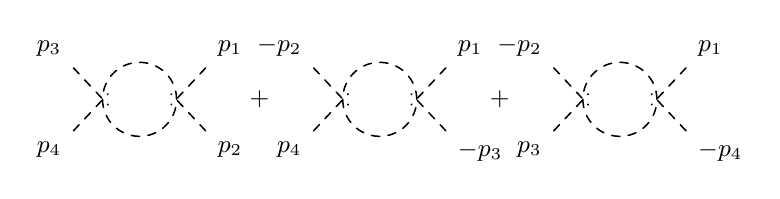
\begin{tikzpicture}[x=1cm,y=1cm,baseline=-.4ex,line cap=round,
  every node/.style={font=\small}]
  % Three one-loop bubbles.  At each vertex the two external legs cross,
  % overshooting slightly into the loop, exactly as in the source.
  \foreach \x in {0,3.05,6.10} {
    \draw[BanksNLoop] (\x,0) circle (.47);
    \draw[BanksNLeg] (\x-.84,.40) -- (\x-.40,-.07);
    \draw[BanksNLeg] (\x-.84,-.40) -- (\x-.40,.07);
    \draw[BanksNLeg] (\x+.84,.40) -- (\x+.40,-.07);
    \draw[BanksNLeg] (\x+.84,-.40) -- (\x+.40,.07);
  }
  \node at (1.525,0) {$+$};
  \node at (4.575,0) {$+$};
  % s-channel
  \node[anchor=south east] at (-.87,.42) {$p_3$};
  \node[anchor=north east] at (-.87,-.42) {$p_4$};
  \node[anchor=south west] at (.87,.42) {$p_1$};
  \node[anchor=north west] at (.87,-.42) {$p_2$};
  % t-channel
  \node[anchor=south east] at (2.18,.42) {$-p_2$};
  \node[anchor=north east] at (2.18,-.42) {$p_4$};
  \node[anchor=south west] at (3.92,.42) {$p_1$};
  \node[anchor=north west] at (3.92,-.42) {$-p_3$};
  % u-channel
  \node[anchor=south east] at (5.23,.42) {$-p_2$};
  \node[anchor=north east] at (5.23,-.42) {$p_3$};
  \node[anchor=south west] at (6.97,.42) {$p_1$};
  \node[anchor=north west] at (6.97,-.42) {$-p_4$};
\end{tikzpicture}

  \caption{s-, t- and u-channel diagrams for the one-loop four-point function.}
  \label{fig:9.4}
\end{figure}

% BANKS-SOURCE: pdf=167 print=157 kind=prose
which are used to cancel out loop corrections to the physical mass and coupling
and the normalization of the single-particle matrix element of the field. One
can define an analogous counterterm method for any choice of definition of the
renormalized parameters.

Now let us consider loop corrections to the quantum action. Since we are using a
normal ordered interaction, there is no one-loop correction to the 1PI two-point
function. For $n\geq5$ the one-loop correction to the $n$-point function is
cut-off-independent (the loop integrals are finite). The one-loop, 1PI Euclidean
four-point function is given by a sum of three diagrams (Figure~\ref{fig:9.4}).

They all have the form
% BANKS-SOURCE: pdf=167 print=157 kind=equation
\[
  \frac{1}{2}\lambda_0^2\int\frac{\dd^{d_{\mathrm{reg}}}p}{(2\pi)^{d_{\mathrm{reg}}}}
  \frac{1}{(p^2+m_0^2)[(p-q)^2+m_0^2]},
\]
where $q=p_1+p_2$, $p_1-p_3$, $p_1-p_4$, in the three different diagrams. The
combinatoric factor $\frac12$ comes from the symmetry of the two internal lines
in the diagram.

To this order, the 1PI two-point function of $\phi$ is $Z^{-1}(p^2+m^2)$. Since
it is independent of $\lambda_0$ it must reproduce the physics of the free
theory. We identify $Z=1$ and $m_0^2=m^2$, the physical mass of the free
particle. Thus, any divergence in the four-point function is related to the
cut-off dependence of $\lambda_0$. In order to get explicit expressions, we have
to decide how we are going to cut off the integral. The general theory of the RG
assures us that we can do this any way we like. The functional form of the bare
parameters in terms of renormalized parameters and the cut-off will depend on the
cut-off procedure, as well as on the definition of the renormalized parameters
(usually called the \emph{renormalization scheme}).

We will use the dimensional regularization scheme. Rewrite the propagators using
the Schwinger proper-time trick,
% BANKS-SOURCE: pdf=167 print=157 kind=equation
\[
  \frac{1}{P}=\int\dd s\,\ee^{-sP},
\]
and then do the Gaussian momentum integrals, using the formula
% BANKS-SOURCE: pdf=167 print=157 kind=equation
\[
  \int\frac{\dd^{d_{\mathrm{reg}}}p}{(2\pi)^{d_{\mathrm{reg}}}}\,\ee^{-sp^2}
  =\left(\frac{\pi}{4s}\right)^{d_{\mathrm{reg}}/2}.
\]
The result is
% BANKS-SOURCE: pdf=167 print=157 kind=equation
\[
  \frac{1}{2}\int_0^\infty s\,\dd s\int_0^1\dd x
  \left(\frac{\pi}{4s}\right)^{d_{\mathrm{reg}}/2}
  \ee^{-s[x(1-x)q^2+m^2]}.
\]
We have arrived at this formula by making the change of variables
$s_1=(1-x)s$, $s_2=xs$, where $s_1$ is the Schwinger parameter for
$(p^2+m^2)^{-1}$ and $s_2$ the parameter for the propagator that depends on
external momenta.

% BANKS-SOURCE: pdf=168 print=158 kind=source-page
% BANKS-SOURCE: pdf=168 print=158 kind=prose
Note that, at this point, the space-time dimension $d_{\mathrm{reg}}$ is just a
parameter, and can take on arbitrary complex values in the analytic
continuation. We will see that the integrals actually define analytic
functions of $d_{\mathrm{reg}}$, with poles at $d_{\mathrm{reg}}=4$.
% BANKS-SOURCE: pdf=168 print=158 kind=equation
Assuming that this is so, we can simplify things by rescaling the $s$ variable to
make the argument of the exponent simply $s$. We obtain
% BANKS-SOURCE: pdf=168 print=158 kind=equation
\[
  \frac{1}{2}\int_0^\infty s\,\dd s\int_0^1\dd x
  \left(\frac{\pi}{4s}\right)^{d_{\mathrm{reg}}/2}
  [x(1-x)q^2+m^2]^{d_{\mathrm{reg}}/2-2}\ee^{-s}.
\]
The $s$ integral now gives $\Gamma(2-d_{\mathrm{reg}}/2)$, which has a pole at
$d_{\mathrm{reg}}=4$. Note that, if we take derivatives with respect to $q^2$ or $m^2$, we
bring down a power of $(d_{\mathrm{reg}}-4)$, which cancels out the pole. Thus, the divergence
resides only in the constant term.

The tree-level 1PI four-point function is just $\lambda_0$, so, if we write
$\lambda_0=\lambda+\lambda^2f(d_{\mathrm{reg}})$ where $\lambda$ is finite, and $f$ has a pole
which cancels out the pole in the one-loop computation, then we will get a finite
answer as a function of $\lambda$.

We continue to discuss the renormalization program by turning to the two-loop,
two-point function.\footnote[10]{We will not calculate the two-loop 1PI four-point
function, which should be done to complete the renormalization program. The
interested reader should try it, and will see that the calculation is quite
simple.}
There is one graph, Figure~\ref{fig:9.5}, with a symmetry factor $1/3!$. It can
be evaluated by introducing three Schwinger parameters,
% BANKS-SOURCE: pdf=168 print=158 kind=equation
\[
  \begin{aligned}
  \Sigma_2(q)&=\frac{\lambda_0^2}{(2\pi)^{2d_{\mathrm{reg}}}3!}
  \int\dd s_1\,\dd s_2\,\dd s_3
  \int\dd^{d_{\mathrm{reg}}}p_1\,\dd^{d_{\mathrm{reg}}}p_2\\
  &\quad\times\left[\ee^{-s_1(p_1^2+m_0^2)}\ee^{-s_2(p_2^2+m_0^2)}
  \ee^{-s_3((q-p_1-p_2)^2+m_0^2)}\right].
  \end{aligned}
\]
We do the momentum integrals using the Gaussian integral formula
% BANKS-SOURCE: pdf=168 print=158 kind=equation
\[
  \int\dd^{d_{\mathrm{reg}}}p\,\ee^{-ap^2+bp}
  =\left(\frac{\pi}{a}\right)^{d_{\mathrm{reg}}/2}\ee^{b^2/(4a)}.
\]
To display the result, I will write the integrand as it appears after each
Gaussian integral. We will change variables to $s_i=sx_i$, $\sum x_i=1$, with
$\dd s_1\,\dd s_2\,\dd s_3=s^2\dd s\,\dd x_1\,\dd x_2\,\dd x_3
\delta(1-\sum x_i)$. I will also omit the prefactor
$\lambda_0^2/[(2\pi)^{2d_{\mathrm{reg}}}3!]$. After the $p_1$ integration we obtain
% BANKS-SOURCE: pdf=168 print=158 kind=equation
\[
  s^2\left(\frac{\pi}{s(x_1+x_3)}\right)^{d_{\mathrm{reg}}/2}
  \ee^{-sm_0^2}
  \ee^{-sp_2^2\frac{x_1x_2+x_2x_3+x_1x_3}{x_1+x_3}}
  \ee^{2sp_2q\frac{x_1x_3}{x_1+x_3}}
  \ee^{-sq^2\frac{x_1x_3}{x_1+x_3}}.
\]

% BANKS-SOURCE: pdf=168 print=158 kind=figure id=9.5
\begin{figure}[htbp]
  \centering
  % BANKS-SOURCE: pdf=168 print=158 kind=figure id=9.5
% The single two-loop "sunset" graph: two vertices joined by three
% internal lines, with the external momentum p entering on the right.
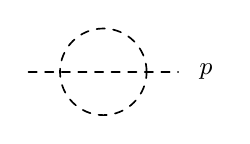
\begin{tikzpicture}[x=1cm,y=1cm,baseline=-.4ex,line cap=round]
  \draw[line width=.6pt,dash pattern=on 3pt off 3pt] (-0.95,0)--(0.95,0);
  \draw[line width=.6pt,dash pattern=on 3pt off 3pt] (0,0) circle (.55);
  \node[anchor=west,font=\small] at (1.10,0) {$p$};
\end{tikzpicture}

  \caption{Two-loop mass and wave-function renormalization.}
  \label{fig:9.5}
\end{figure}

% BANKS-SOURCE: pdf=169 print=159 kind=source-page
After the $p_2$ integral, this simplifies to
% BANKS-SOURCE: pdf=169 print=159 kind=equation
\[
  s^2\left(\frac{\pi}{s}\right)^{d_{\mathrm{reg}}}
  \left(\frac{1}{x_1x_2+x_2x_3+x_1x_3}\right)^{d_{\mathrm{reg}}/2}
  \ee^{-s\left(m_0^2+q^2\frac{x_1x_2x_3}{x_1x_2+x_2x_3+x_1x_3}\right)}.
\]
Next, we do the $s$ integral, which produces a factor of
% BANKS-SOURCE: pdf=169 print=159 kind=equation
\[
  \Gamma(3-d_{\mathrm{reg}})\left(q^2\frac{x_1x_2x_3}{x_1x_2+x_2x_3+x_1x_3}
  +m_0^2\right)^{d_{\mathrm{reg}}-3}.
\]
The only divergence we can get in the $x_i$ integrals comes at points where two
of the variables approach $0$ while the other is forced to be $1$ by the delta
function. Near such limits, the integrand behaves like
$\dd x\,\dd y\,W/(x+y)^{d_{\mathrm{reg}}/2}$,
where $x,y$ are the two variables which go to zero. The coefficient $W$ is
independent of $q^2$ because the coefficient which multiplies $q^2$ vanishes at
the dangerous points. Thus, the answer contains single and double poles at
$d_{\mathrm{reg}}=4$, which are momentum-independent, and a single pole proportional to $q^2$.

The divergent part of the effective action coming from this diagram is given by
% BANKS-SOURCE: pdf=169 print=159 kind=equation
\[
  \Gamma_{\mathrm{div}}=\frac{\lambda_0^2}{3!(4\pi)^{d_{\mathrm{reg}}}}
  \Gamma(3-d_{\mathrm{reg}})
  \int\dd^{d_{\mathrm{reg}}}x\left[(\partial_\mu\phi)^2I_1+m_0^2\phi^2I_2\right].
\]
$I_{1,2}$ are given by the following parametric integrals:
% BANKS-SOURCE: pdf=169 print=159 kind=equation
\[
  \begin{aligned}
  I_1&=\int_0^1\dd x\int_x^1\dd y\,
  \frac{x(y-x)(1-y)}{[x(y-x)+y(1-y)]^3},\\
  I_2&=\int_0^1\dd x\int_x^1\dd y\,
  \frac{1}{[x(y-x)+y(1-y)]^{d_{\mathrm{reg}}/2}}.
  \end{aligned}
\]
$I_1$ is finite, while $I_2$ has a single pole at $d_{\mathrm{reg}}=4$. The minimal
subtraction (MS) renormalization scheme is defined by keeping only the pole
terms in the relation between renormalized bare fields and parameters. In
defining the divergent part of the above integrals in the MS scheme, we keep
both the pole and the finite correction in $I_2$, and throw away terms of order
$d_{\mathrm{reg}}-4$. The residues of all poles in $\Gamma_{\mathrm{div}}$ are given by
integrals we can evaluate in terms of elementary functions, but the calculation
is a bit tedious.

\BanksImplicitHook{I-CH09-009}

We have demonstrated that all the divergent terms in the effective action
correspond to one of the three operators $:(\partial_\mu\phi)^2:$, $:\phi^2:$,
and $:\phi^4:$, and therefore expect that cut-off dependence of the coefficients
of these terms in the bare Lagrangian will render the Green functions independent
of the cut-off in the limit that it goes to infinity. That is, a Lagrangian of the
form
% BANKS-SOURCE: pdf=169 print=159 kind=equation
\[
  \mathcal{L}=\frac{1}{2}:\!\left[-(\partial_\mu\phi_0)^2-m_0^2\phi_0^2
  -\frac{\lambda_0}{2\cdot3!}\phi_0^4\right]\!:\,
\]
with appropriate cut-off dependence in $m_0$ and $\lambda_0$, will give finite
Green functions for the field $\phi=Z^{-1/2}\phi_0$, with cut-off-dependent $Z$.
The renormalization procedure consists of tuning the parameters in such a way
that the rescaled field $\phi$ has cut-off-independent Green functions.

% BANKS-SOURCE: pdf=170 print=160 kind=source-page
Our calculations have shown that
% BANKS-SOURCE: pdf=170 print=160 kind=equation
\[
  \Gamma_{\mathrm{div}}[\phi]
  =\frac{a}{2}\lambda_0^2(\partial_\mu\phi_0)^2
  +\frac{b}{2}\mu^2\lambda_0^2\phi_0^2
  +\frac{c}{3!}\lambda_0^2\phi_0^4,
\]
where
% BANKS-SOURCE: pdf=170 print=160 kind=equation
\[
  a=\frac{\lambda_0^2}{3!(4\pi)^{d_{\mathrm{reg}}}}
  \Gamma(3-d_{\mathrm{reg}})I_1,
  \qquad
  b=\frac{\lambda_0^2}{3!(4\pi)^{d_{\mathrm{reg}}}}
  \Gamma(3-d_{\mathrm{reg}})\frac{2m_0^2}{\mu^2}I_2,
  \qquad
  c=\frac{3}{16\pi^2(d_{\mathrm{reg}}-4)}.
\]
We note that, in $d_{\mathrm{reg}}$ dimensions, the coupling $\lambda_0$ has dimensions
$(\text{mass})^{4-d_{\mathrm{reg}}}$. To eliminate the cut-off dependence in the quantum
action, we define $\lambda_0=\mu^{4-d_{\mathrm{reg}}}(\lambda+A\lambda^2)$,
$m_0^2=m^2+B\mu^2\lambda^2$, and $\phi_b=\sqrt{Z}\phi$, with
$Z=1+z_\phi\lambda^2$. The parameters $\lambda$ (which is taken to be dimensionless)
and $m^2$ are held fixed as we take away the cut-off $d_{\mathrm{reg}}\to4$, and the $\phi$ field
should have a finite quantum action. In these formulae, we have introduced a
parameter $\mu^2$, called the \emph{renormalization scale} in dimensional
regularization. It is necessary to rewrite functions of the dimensional constant
$\lambda_0$ in terms of the dimensionless parameter $\lambda$.

The relevant and marginal terms in the Euclidean quantum action are
written with $(\partial_\mu\phi)^2$ positive; the Lorentzian kinetic terms
above use the mostly-plus convention.
% BANKS-SOURCE: pdf=170 print=160 kind=equation
\[
  \frac{1}{2}(1+a\lambda_0^2)(\partial_\mu\phi_0)^2
  +\frac{1}{2}(m_0^2+bm_0^2\lambda_0^2)\phi_0^2
  +\frac{\lambda_0}{3!}(1+c\lambda_0)\phi_0^4.
\]
We write this in terms of renormalized fields and parameters, dropping terms of
higher order than $\lambda^2$. The coefficient of the kinetic term is
$(1+z_\phi\lambda^2)(1+a\lambda^2)\simeq1+(z_\phi+a)\lambda^2$. That of the mass term is
% BANKS-SOURCE: pdf=170 print=160 kind=equation
\[
  (1+z_\phi\lambda^2)(m^2+B\mu^2\lambda^2+b\mu^2\lambda^2)
  \simeq m^2+\lambda^2(z_\phi m^2+(B+b)\mu^2),
\]
while the quartic term has coefficient
% BANKS-SOURCE: pdf=170 print=160 kind=equation
\[
  \frac{\lambda}{3!}\bigl(1+(A+2z_\phi+c)\lambda\bigr).
\]
We first choose $z_\phi+a$ to have a cut-off-independent limit. Then $B$ can be
chosen so that $z_\phi m^2+(B+b)\mu^2$ has a cut-off-independent limit. Finally, $A$
is chosen so that the renormalized quartic coupling is finite.

Note that this procedure does not introduce cut-off dependence into the
$o(\lambda^2)$ finite part of the 1PI action. $\Gamma_{\mathrm{finite}}$ is
initially written in terms of the bare parameters and bare fields, and is of
order $\lambda_0\sim\lambda$. When written in terms of renormalized fields and
parameters, it has divergent pieces, but they are of order $\lambda^3$ and
higher. The basic claim of renormalization theory is that these terms cancel out
exactly against sub-divergences in higher-order Feynman graphs. The combinatorics
of this appears daunting, but a proof that it works was carried out by a number
of authors. Our Wilsonian approach through the exact RGE assures us that it
\emph{must} work.

It is worthwhile pausing here to remark on the precise connection between our
discussion of the exact Wilsonian RGE and dimensional regularization. In the
context of the RGE we have remarked that we can easily replace one cut-off by
another, changing the kinetic function $K(p)$ or going over to a lattice cut-off,
without changing the qualitative nature of the RG flow, its fixed points, or the
dimensions of operators at those points. Dimensional regularization is just
another way of cutting off the divergences,

% BANKS-SOURCE: pdf=171 print=161 kind=prose
albeit one that is defined only perturbatively. We should expect to be able to
perform renormalized computations near the Gaussian fixed point using DR, with
couplings that are related to those of the Wilsonian RGE by a finite
redefinition
% BANKS-SOURCE: pdf=171 print=161 kind=equation
\[
  \lambda_{\rm DR}=\lambda_W+\sum k_n\lambda_W^n.
\]

Returning to our computation, we note that requiring the quantum action to be
finite does not determine the parameters $A$, $B$, $D$ uniquely. Each choice of
this finite ambiguity determines another way of parametrizing the renormalized
field theory, called a renormalization scheme. One conceptually simple scheme
called on-shell renormalization chooses the ambiguity so that $m^2$ is exactly
the position of the zero in the 1PI two-point function, and the vacuum to
one-particle matrix element of the renormalized field is 1; $-\ii\lambda$ is
then chosen to be the value of the invariant $2\to2$ scattering amplitude at
the symmetric point in momentum space, $s=4m^2$, $t=u=0$.

This is not always the most convenient scheme. It requires us to be able to
find the masses of particles in perturbation theory. In QCD and other
asymptotically free gauge theories this is impossible. It also ties our
renormalization scheme to quantities in Minkowski space. For many purposes, a
Euclidean renormalization scheme, which is not directly tied to physical
masses, is better. For perturbative calculations, the most efficient scheme is
the so-called $\overline{\rm MS}$ or modified minimal subtraction scheme. This
exploits the way in which dimensional regularization isolates cut-off
dependence in terms of poles in analytic functions. The minimal subtraction
scheme is defined by letting $A$, $B$, $z_\phi$, and analogous higher-order
coefficients have precisely the poles in $d_{\mathrm{reg}}-4$ that they need in order to give
finite Green functions. No finite parts are admitted in the definition of
these coefficients. It turns out that this prescription leads to a
proliferation of transcendental numbers (related to the derivative of the
Euler gamma function at $t=1$) in formulae for finite amplitudes in terms of
the MS parameters. The $\overline{\rm MS}$ scheme allows specific finite parts
in $A$, $B$, $z_\phi$, etc., which get rid of these transcendentals. The reader is
urged to consult the book by Peskin and Schroeder \cite{banks-ref-33} for many
examples of computations in the $\overline{\rm MS}$ scheme.
